\chapter{I Was Broke, Found God, and Now I Make \$15M/Year}

This interview is not a blackboard lecture, but it does contain a real mathematical spine. We are led from credibility, reversal, and promise into a sequence of sharper claims about attention, money, survival, eras of wealth creation, sales, assets, mentorship, and trust. The useful way to read it is not as a bag of motivational lines, but as a small system: what we focus on changes what we build, what we build changes what produces income, and what we withdraw too early weakens the whole structure. We will therefore keep close to the order of the conversation and formalize only those relations that the interview itself clearly supports.

\section{Prologue: Proof, Reversal, and the Promise}

The opening montage is doing serious structural work. Before the golf-course conversation begins, the host compresses an earlier street interview into a credentialing sequence: Myron Golden is a consultant and entrepreneur, he has made \$15 million in a single year, he has been broke, then rich, then broke again, and he now claims to have arranged his affairs so that the collapse does not repeat. The prologue adds one more axis immediately: ``I trust God.'' The later discussion will return to this line, but the important point at the start is that the interview wants us to treat commercial success, personal reversal, and theological confidence as parts of a single life.

That opening is then amplified by virality. The host reports roughly 150 million views across social media and pivots from proof to promise: Golden has invited the team to a private golf course in Tampa, Florida to give a ``blueprint'' for becoming a multimillionaire and for learning to sell and market like a \$15 million-per-year entrepreneur. In other words, the interview is framed as a course in applied commercial reasoning. The conversation will move quickly, but the order matters: first authority, then the promise of instruction, then the principles.

\section{Intention, Distraction, and the Function of Money}

The first substantive principle is a filter on attention. Asked what the wealthiest people do differently, Golden does not begin with tactics, asset classes, or marketing channels. He begins with a sorting rule.

\begin{definition}
For any activity \(a\), we may encode Golden's first distinction as
\begin{align}
I(a)=1 &\iff a \text{ moves the needle in our favor},\\
D(a)=1 &\iff a \text{ does not move the needle in our favor}.
\end{align}
Here \(I(a)\) records intention and \(D(a)\) records distraction.
\end{definition}

The host initially tries to translate this into a diversification thesis, but Golden resists that reading. Diversifying, he says, is a different conversation. The point here is prior to portfolio theory. We first decide whether a unit of attention belongs in the set of activities that advance the objective at hand. Only after that do we discuss how many channels, holdings, or strategies we might rationally employ.

Once attention is filtered, the interview immediately asks a second question: what do wealthy people think money is \emph{for}? Here the lecture becomes especially clean. Let \(M\) denote money viewed not as quantity, but as an object to which one assigns a primary function. Then the interview offers the following classification:
\begin{align}
\text{Poor:}\quad & M \mapsto \text{pay bills},\\
\text{Middle class:}\quad & M \mapsto \text{maintain credit and status consumption},\\
\text{Rich:}\quad & M \mapsto \text{turn money into more money}.
\end{align}

This is a strong claim, and it is not meant merely as a sociological insult. It is a change of operator meaning. The issue is not how much money one has, but which transformation one expects money to perform. If money is assigned to bill service, it disappears into maintenance. If it is assigned to status, it disappears into display. If it is assigned to reproduction, it is routed into a mechanism that seeks more of itself.

Golden then tightens the mechanism further. Money does not multiply simply because we want it to. It multiplies when we learn to perceive what is valuable to other people. The wealth chain, in the lecture's own order, is therefore something like
\begin{equation}
\text{solve problems for others} \rightarrow \text{income} \rightarrow \text{retained capital} \rightarrow \text{assets} \rightarrow \text{more income}.
\end{equation}
He explicitly rejects the self-enclosed stance in which we stare only at our own shortage. One solves one's money problem by solving somebody else's problem, and by focusing on their difficulty rather than on one's own immediate hunger.

\section{Losing Money: Low Burn and Structural Survival}

The interview then tests whether these principles survive contact with biography. Golden corrects himself when asked about his first million, finally settling on age \(45\), but he also says that before that he had already made a million dollars per year for a couple of years in a row and then lost all of his money. This transition matters. We are no longer discussing the acquisition of revenue in the abstract. We are discussing the stability of a financial system after success has begun.

His answer has two parts. First, there were tragedies. Second, and more analytically useful for us, he upgraded his lifestyle too soon. That yields the operative warning: when riches increase, so do they that consume them. The principle is not anti-consumption as such; it is anti-fragility. If inflow rises and fixed withdrawals rise with it, then the system acquires a larger appetite exactly when it should be acquiring reserves.

Let \(X_t\) denote current inflow, \(C_t\) lifestyle consumption or withdrawal, \(S_t:=X_t-C_t\) retained surplus, and \(W_t\) total retained wealth or working capital at time \(t\). Golden's concrete benchmark is blunt:
\begin{equation}
C_t \le 0.1X_t.
\end{equation}
He states this as ``live off of \(10\%\) of your revenue or \(10\%\) of your income.'' We should not pretend the number \(0.1\) is an optimized theorem; it is a lecture rule. But it is a useful one, because it forces us to separate the cash that sustains the person from the cash that sustains the compounding process.

A cautious bookkeeping model of the point is
\begin{equation}
W_{t+1}=W_t+\Pi_t-C_t,
\end{equation}
where \(\Pi_t\) denotes retained earnings plus returns that remain in the structure. If we write, more explicitly,
\begin{equation}
W_{t+1}=(1+r)W_t+S_t,\qquad S_t:=X_t-C_t,
\end{equation}
then we are not claiming that Golden wrote down this recurrence; we are simply making his compounding intuition precise.

\paragraph{Worked example.}
Suppose, in the spirit of his own numbers, that monthly inflow is fixed at
\[
X_t \equiv 50{,}000,
\]
and the low-burn rule is enforced at
\[
C_t = 0.1X_t = 5{,}000.
\]
Then retained surplus is
\[
S_t = X_t-C_t = 45{,}000.
\]
If we now use the update rule
\[
W_{t+1}=(1+r)W_t+45{,}000,
\]
we get
\begin{align}
W_1 &= (1+r)W_0+45{,}000,\\
W_2 &= (1+r)W_1+45{,}000
     = (1+r)^2W_0+(2+r)\cdot 45{,}000,\\
W_3 &= (1+r)W_2+45{,}000
     = (1+r)^3W_0+\bigl(3+3r+r^2\bigr)\cdot 45{,}000.
\end{align}
Hence, in closed form,
\begin{equation}
W_n=(1+r)^nW_0+45{,}000\sum_{k=0}^{n-1}(1+r)^k.
\end{equation}

The lecture never speaks in these symbols, but the argument is exactly this: if we withdraw less, then the amount that remains inside the machine becomes larger, and once the base becomes larger, the future increments grow faster. This is why Golden insists that there is nothing wrong with buying things, but that the business must be sustained first. The saying he gives, ``stay small enough, long enough, and you'll be big enough soon enough,'' is a verbal version of the same recurrence.

\section{Economic Eras, AI, and the Rejection of Deadline Goals}

The next pivot widens the frame. Asked what industry he would enter right now, Golden answers immediately: something to do with AI. The reason he gives is not a detailed technology forecast, but a regime argument. Wealth, he says, migrates across sectors, and when it does so a new economic era is introduced. In rough historical order, the interview offers the following sequence.

\begin{figure}[h]
\centering
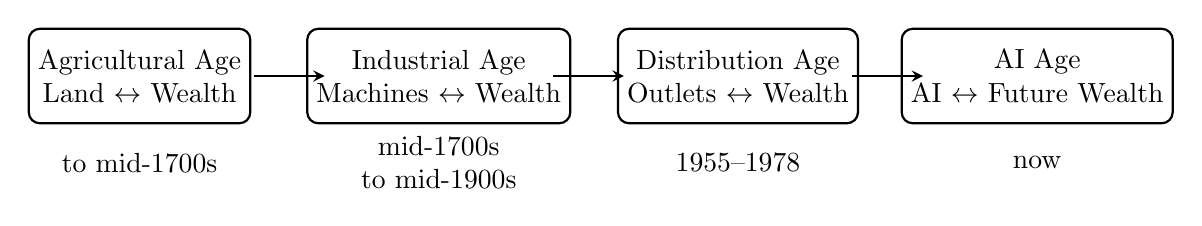
\begin{tikzpicture}[>=stealth,thick]
\node[draw,rounded corners,align=center,minimum width=2.7cm,minimum height=1.2cm] (a) at (0,0) {Agricultural Age\\Land \(\leftrightarrow\) Wealth};
\node[draw,rounded corners,align=center,minimum width=2.7cm,minimum height=1.2cm] (b) at (3.8,0) {Industrial Age\\Machines \(\leftrightarrow\) Wealth};
\node[draw,rounded corners,align=center,minimum width=2.7cm,minimum height=1.2cm] (c) at (7.6,0) {Distribution Age\\Outlets \(\leftrightarrow\) Wealth};
\node[draw,rounded corners,align=center,minimum width=2.7cm,minimum height=1.2cm] (d) at (11.4,0) {AI Age\\AI \(\leftrightarrow\) Future Wealth};
\draw[->] (1.45,0) -- (2.35,0);
\draw[->] (5.25,0) -- (6.15,0);
\draw[->] (9.05,0) -- (9.95,0);
\node[align=center] at (0,-1.1) {to mid-1700s};
\node[align=center] at (3.8,-1.1) {mid-1700s\\to mid-1900s};
\node[align=center] at (7.6,-1.1) {1955--1978};
\node[align=center] at (11.4,-1.1) {now};
\end{tikzpicture}
\caption{The transcript-derived sequence of wealth regimes. The chronology is kept in the rough form in which it is spoken.}
\end{figure}

Again, we should not over-interpret the figure. This is not a full economic history. It is the structural claim that each era has a dominant leverage. In the present era, Golden's thesis is that those who entered AI early, or even now, will create the wealth of the future.

The host then asks a classic pressure question: if one had to start from zero and make a million dollars in \(90\) days, what would one do? Golden refuses the premise. This refusal is not evasive. It is a second formal move.

\begin{definition}
Golden's definition of a goal is
\begin{equation}
G := O + \tau,
\end{equation}
where \(O\) is an objective and \(\tau\) is a deadline.
\end{definition}

The reason he rejects the challenge is that the deadline term \(\tau\) is often not under our control. He uses a farmer analogy: one does not command \(7\) million ears of corn by next Wednesday if the seasons will not cooperate. Hence the lecture replaces deadline-goals with two more limited objects,
\begin{align}
O_{\mathrm{in}} &: \text{objective for inputs},\\
O_{\mathrm{out}} &: \text{objective for outcomes},
\end{align}
while leaving the hard deadline unforced if it depends on processes outside our control.

This part of the interview is easy to trivialize, but it should not be. The point is not that we abandon ambition. The point is that uncontrolled deadlines generate false negative feedback. They induce the feeling of failure before the process has actually closed. Golden is trying to remove the self-imposed term that corrupts persistence.

\section{Sales as Value Revelation}

The conversation then narrows again, this time into sales. Asked whether he is a good salesman, Golden answers without false modesty: one of the best in the world. The very next question therefore asks for the distinguishing rule, and again the answer is cleaner than many systems of technique: he only sells people things they desire to buy.

This immediately removes the common caricature of sales as coercion. It also lets us connect the early slogan, ``where attention goes, revenue flows,'' to the later mechanics of conversion.

\begin{definition}
In the lecture's own spirit, sales is the uncovering of value clearly enough that a buyer is happy to exchange money for it.
\end{definition}

The process can be summarized as
\begin{equation}
\text{Attention} \rightarrow \text{Trust} \rightarrow \text{Transaction} \rightarrow \text{Investment}.
\end{equation}
At the beginning of the chain, buyers do not yet know that we exist. Golden's recommendation is therefore not ``push harder,'' but ``become findable.'' There are already people who would love to buy what one would love to sell, if only the two sides were made visible to one another.

Several consequences follow. First, sales is not primarily about talking reluctant strangers into purchase. Second, pricing is part of market selection. Golden says his coaching is \$40,000 an hour, his mentorship programs and masterminds are in the \$20,000--\$30,000 range, and some offers extend to \$1 million per year. These numbers are not ornamental boasting. They function as filters: they attract the right people and repel the wrong ones. Third, the right problem class matters. The same human energy, he says, can be spent solving a \$5,000 problem or a \$100,000 problem. The difference is not the expenditure of vitality in the abstract, but the nature of the buyer and the magnitude of the solved problem.

This explains the later one-to-many selling story as well. A large single-day result, like the reported \$5.5 million day, is not magic at the instant of the pitch. The pitch sits atop accumulated attention and relationship. The host's dating analogy here is useful: one does not walk up to a stranger and propose marriage. One builds rapport first. In the same way, premium selling is not a single move; it is the late stage of a long attention-and-trust process.

\section{Changing the Family Trajectory}

The interview now reaches its sharpest tension. After the sales discussion, the host turns the conversation back toward origin and asks how Golden changed his family's trajectory.

\subsection{Question \& Answer}

The question is posed against a familiar slogan: the rich get richer, the poor get poorer. Golden's first move is not yet the answer. It is a correction.
\begin{equation}
\text{correlation} \neq \text{causation}.
\end{equation}
The rich getting richer and the poor getting poorer may both be true statements, he says, but they do not by themselves explain why one causes the other. That is an important logical cleanup. It prevents the chapter from treating a social slogan as a mechanism.

His answer then has motive and mechanism. The motive is personal and simple: he hated being poor. The mechanism is learned and structural: he began to do the things rich people do instead of the things poor people do. The most compact form of the principle is the line he attributes to Daniel Priestley:
\begin{equation}
A \rightarrow Y,
\end{equation}
that is, income follows assets.

This does not yet mean that \(A\) is a smooth measurable function in any strict analytic sense. It means that the interview's center of gravity shifts from labor-hours and bill-paying to the acquisition and construction of assets. Golden explicitly says that he stopped focusing on working hard, on eight hours of work for eight hours of pay, and on paying bills. He started focusing on putting more assets in the asset column.

\begin{figure}[h]
\centering
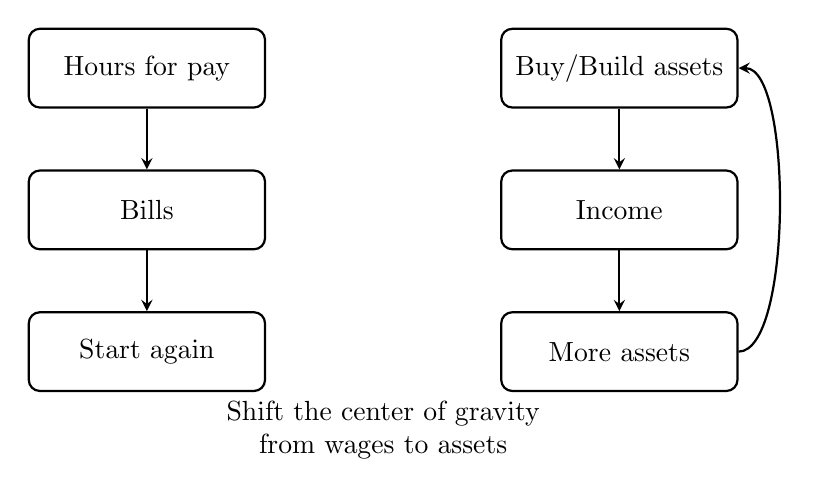
\begin{tikzpicture}[>=stealth,thick]
\node[draw,rounded corners,align=center,minimum width=3.0cm,minimum height=1cm] (l1) at (0,0) {Hours for pay};
\node[draw,rounded corners,align=center,minimum width=3.0cm,minimum height=1cm] (l2) at (0,-1.8) {Bills};
\node[draw,rounded corners,align=center,minimum width=3.0cm,minimum height=1cm] (l3) at (0,-3.6) {Start again};

\node[draw,rounded corners,align=center,minimum width=3.0cm,minimum height=1cm] (r1) at (6,0) {Buy/Build assets};
\node[draw,rounded corners,align=center,minimum width=3.0cm,minimum height=1cm] (r2) at (6,-1.8) {Income};
\node[draw,rounded corners,align=center,minimum width=3.0cm,minimum height=1cm] (r3) at (6,-3.6) {More assets};

\draw[->] (l1) -- (l2);
\draw[->] (l2) -- (l3);

\draw[->] (r1) -- (r2);
\draw[->] (r2) -- (r3);
\draw[->] (r3.east) .. controls (8.2,-3.6) and (8.2,0) .. (r1.east);

\node[align=center] at (3,-4.6) {Shift the center of gravity\\from wages to assets};
\end{tikzpicture}
\caption{A transcript-derived contrast between wage-centered and asset-centered thinking.}
\end{figure}

The interview then makes the asset language concrete. One can buy assets, and one can build assets. Books are an example of a built asset: written once, paid every month thereafter. Real estate options and crypto are named as present investments. But Golden also says that the most important investment he ever made was in his own mind. That belongs in the same section because it answers a subtle question: who or what produces the capacity to build the next asset? His answer is that learned capability is itself part of the asset-generating apparatus.

\section{Mentorship, Scale, Service, and Trust}

The next major move is epistemic. Asked how much he has spent on mentorship, Golden answers: about \$1.7 million, counting books, courses, coaching programs, and the rest. The point of the number is not extravagance. It is leverage. Mentorship is the ultimate shortcut because another person has already spent a lifetime discovering a path, and one may buy access to the structure of that discovery. The lecture's most useful phrasing here is that the real obstacle is not only what we do not know, but what we do not know we do not know. Mentorship exposes that hidden layer.

His first mentor, Jerry, taught him how to sell from stage, one-to-many. The importance of this anecdote is not merely technical. Golden says he did not even believe the method would work until he used it. In other words, applied obedience precedes intuitive certainty. Only after the method cashes out does the mind revise its sense of the possible.

A second mentorship story does even more work. At a seminar, after Golden testified that he had gone from trash man at \$6.25 an hour to someone making \$30,000 a month, Robert G. Allen told him he was doing well and was on the path to making some really big money. The shock, as Golden reports it, is conceptual: \( \$30{,}000 \) a month suddenly appears not as the finish line, but as a lower tier. This is how the lecture moves from asset logic to scale logic. Wealth is again framed as perception before possession. One must learn to perceive bigger structures already present in the world.

After a promotional interlude, the interview returns to advanced selling and room access. The advice is blunt: if one wants to get in the room, one pays to get in the room, and one gets paid on the way out. Golden describes joining a mastermind as the broke person in the room and discovering that people financially far ahead of him still saw value in his ideas. The resulting correction is subtle and important: he had long been selling to people who needed what he had, rather than to people who wanted it and could pay for it.

This leads to the final, fully developed sales sequence of the interview. Sell to rich people if the objective is to get rich. Solve expensive problems. Place price transparency early enough that the wrong audience self-selects out. Do not think of sales as extracting money, but as delivering value such that payment becomes natural. That is why lowering price is not automatically the right response to resistance. One may instead raise revealed value.

The last movement of the chapter returns to the line planted in the prologue: trust in God. Golden's answer is not abstract metaphysics. It is testimonial. He says he trusts God because God has never lied to him, because what God says in the Bible has proven itself not merely true but truth. We need not convert this into a neutral doctrine; in these notes we simply record that for Golden the financial, pedagogical, and spiritual strands are not separable. A biblical financial lesson, as he gives it, is that the blessing of the Lord makes rich and adds no sorrow with it. Another is that greatness comes through service: one can be great even if not unusually gifted, provided one is willing to serve enough people. Thus the chapter closes where much of it has been heading all along: wealth is ultimately linked to mass service, gratitude, and the refusal to mistake gift for self-creation.

The last exchange, when the host asks what God has been teaching him in the last year, answers the whole interview from above. Life is short. Pack it with real experience. Live with gratitude. Everything good is gift. In the architecture of the interview, that is not an appendix. It is the final frame that tells us how Golden interprets the rest.

\section{Summary}

The interview begins as proof, becomes a blueprint, and ends as a theology of wealth. Along the way it gives us a small but coherent system. First, filter attention: intention moves the needle, distraction does not. Second, redefine the function of money: not merely bill service, but the production of more money. Third, protect the system with low burn, because early consumption can destroy the very compounding process that success has finally made possible. Fourth, understand the regime in which wealth is currently forming. Fifth, treat sales as value revelation, not coercion. Sixth, escape poverty by shifting from wages to assets. Seventh, use mentorship to expose hidden ignorance and to enlarge the scale of the thinkable.

None of this is presented as pure technique. The lecture keeps turning technique into structure, and structure into posture. Attention, assets, sales, and service are all parts of a larger view in which wealth is produced by solving problems, stabilizing the machine, choosing the right regime, and learning to see abundance where one had previously seen only limit. That is the chapter's final lesson: the system is commercial, but the horizon is moral and spiritual.